\chapter{Processo de desenvolvimento da aplicação}
\label{cha:desenvolvimento}

No capítulo anterior foi apresentado o processo de desenvolvimento
e avaliação dos TCCs no curso de Ciências da Computação da UECE, como este se 
encontra atualmente. 

A partir da visão geral fornecida pelo fluxograma 
da Figura ~\ref{fig:flux_tcc} foi possível definir o comportamento básico 
da aplicação, que é o de aceitar entradas fornecidas pelo estudante e esta seguir sendo aprovada
ou reprovada pelo orientador e pela comissão. Contudo, a aplicação não se 
detém a apenas seguir esse fluxo básico. Ela também possui funcionalidades
de alerta no sistema, para que os envolvidos no processo sejam sempre 
notificados a cada vez que um estudante, orientador ou comissão executem alguma
operação em cima de um projeto.

Neste capítulo discutiremos sobre como o sistema foi modelado e como foi pensado
esse sistema de notificação de eventos.

\section{Escolha das tecnologias}
\subsection{Linguagem de programação}
O PHP é uma linguagem de programação interpretada, multiparadigma, de código aberto, e especialmente
voltada para o desenvolvimento de aplicações para a Web. Possui uma sintaxe que lembra
C, Java e Perl, e se distingue das demais por sua facilidade de aprendizado.
Começou a ser desenvolvida em 1994 por Rasmus Lerdorf, mas o paradigma de orientação
a objetos só foi introduzido a partir da versão 3 (três), amadurecendo na versão 5 (cinco) \cite{PHP, Wiki:PHP}.

O PHP se encontra disponível na grande maioria dos servidores Web e, devido a sua 
facilidade de aprendizado, possui uma vasta comunidade de desenvolvedores. Ele é 
usado em alguns gigantes da Web, como Facebook, Wikipédia e Wordpress \cite{InfoQ:Facebook, Wikipedia:Arquitetura, Wordpress}.

Entre outros fatores, esta linguagem foi escolhida devido a sua difusão, sendo então mais
provável encontrar outros desenvolvedores que possam dar continuidade ao projeto deste trabalho,
adicionando novas funcionalidades ou corrigindo eventuais problemas.

\subsection{Framework}
De acordo com \cite{Minetto}, um framework de desenvolvimento é uma base de onde se pode desenvolver 
algo maior ou mais específico. É uma coleção de códigos-fonte, classes, funções, técnicas e 
metodologias que facilitam o desenvolvimento de novos softwares.

O uso de um framework é essencial para desenvolver uma aplicação rapidamente sem deixar
de seguir boas práticas de programação. Além disso, um programador que conheça um
framework não tem dificuldades para entender o código de outras pessoas, pois o framework obriga todos 
a seguirem as mesmas convenções. Dessa forma o programador que não conhece a aplicação pode se
manter apenas no entendimento da lógica de negócio, sem se perder na arquitetura da aplicação.

Para a aplicação desenvolvida neste trabalho, o framework escolhido foi o Symfony, especialmente 
devido à minha experiência de trabalho com esta ferramenta, visto que eu não queria perder 
tempo para aprender um novo framework. Porém este não foi o único motivo. O Symfony é um 
framework que possui alta aceitação na comunidade PHP, boa documentação, é patrocinado pela 
empresa francesa Sensio Labs, que garante suporte técnico a longo prazo, e tem várias outras 
qualidades que o coloca entre os melhores frameworks PHP, como:

\begin{enumerate}[a.]
\item suporte a PHP 5;
\item suporte a MVC;
\item validação de formulários;
\item extensa documentação;
\item suporte a plugins;
\item geração de código;
\item suporte a ORM e múltiplos bancos de dados;
\item convention over configuration;
\item suporte a testes unitários.
\end{enumerate}

\subsubsection{MVC}
O MVC é um acrônimo para Model-View-Controller, um padrão de projeto que tem como intuito
separar a lógica de negócio, a interface e os modelos de acesso a dados. Essa separação
de conceitos tem como propósito evitar que o código fique difícil de manter e auxilia
significamente no aumento do reuso de código. A Figura ~\ref{fig:diag_mvc} apresenta de maneira
geral a estrutura desse tipo de arquitetura.

\begin{figure}[htbp]
\centering
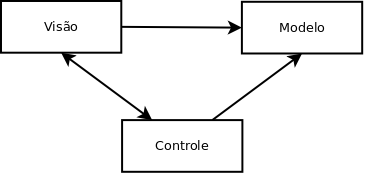
\includegraphics[width=0.5\textwidth]{fig/diagrama_mvc.png}
\caption{Arquitetura MVC}
\label{fig:diag_mvc}
\end{figure}

O modelo de acesso a dados é representado pela camada Model (ou camada de modelo). O modelo 
é um objeto que representa alguma informação sobre o domínio. É um objeto não-visual 
que contém todos os dados e comportamentos outros que não os utilizados 
pela interface \cite{Fowler:2006}.

A camada View (ou camada de visão) representa a interface da aplicação. No trabalho
em questão, ela é a parte em HTML. Esta camada não deve possuir nenhuma lógica de negócio,
detendo-se apenas à captura e exibição de dados.

A camada Controller (ou camada de controle) é a responsável por conectar as outras duas
camadas. O controlador recebe a entrada do usuário (capturado pela visão), manipula o 
modelo e faz com que a visão seja atualizada apropriadamente \cite{Fowler:2006}.




\subsubsection{ORM}
Atualmente a maioria das aplicações é desenvolvida utilizando o paradigma de programação 
orientado a objetos e um banco de dados relacional. Essas aplicações precisam carregar
dados de um banco de dados, criar objetos para representar esses dados em memória,
executar operações em cima destes objetos e depois salvar de volta as alterações no banco.

Ferramentas de mapeamento objeto-relacional (ou ORM) são frameworks que recuperam e persistem
objetos. Seu objetivo é dar suporte à complexa atividade de gerenciar conexões entre
objetos e um banco de dados relacional. A persistência fica transparente ao desenvolvedor,
já que ele não precisa se preocupar com os detalhes de implementação. A ponte entre
objetos e seus relacionamentos é realizada pela ferramenta ORM segundo a especificação 
de mapeamento dos dados \cite{springerlink}.

\subsubsection{Convention over configuration}
Frameworks de propósito geral normalmente necessitam de um ou mais arquivos de configuração
para serem utilizados. Um arquivo de configuração mapeia uma classe e um recurso (uma tabela
no banco de dados) ou um evento (uma requisição web). À medida em que a complexidade das
aplicações cresce, os arquivos de configuração também crescem, tornando-se difíceis de manter \cite{Chen}. 
Para evitar este mal desnecessário, muitos frameworks atualmente procuram seguir o modelo
de desenvolvimento de software de Convenção sobre Configuração (Convention over Configuration).
A idéia é basicamente fazer com que o desenvolvedor só precise definir aquilo que não segue 
uma convenção pré-estabelecida. 

\begin{figure}[!htbp]
\begin{minipage}[t]{0.5\linewidth}
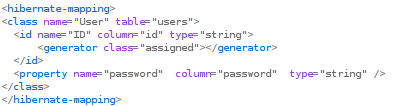
\includegraphics[scale=0.75]{fig/coc_hibernate.png}
\caption{Definição de um mapeamento no Hibernate}\label{fig:coc_hibernate}
\end{minipage} \hfill
\begin{minipage}[t]{0.3\linewidth}
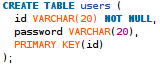
\includegraphics[scale=0.75]{fig/coc_tabela.png}
\caption{Tabela Users no banco de dados}\label{fig:coc_tabela}
\end{minipage}
\end{figure}

A Figura ~\ref{fig:coc_hibernate} apresenta um arquivo de mapeamento para Hibernate,
um framework de mapeamento objeto-relacional para Java. O código da Figura ~\ref{fig:coc_hibernate}
mapeia a classe User com a tabela Users no banco de dados. A tabela Users é descrita 
na Figura ~\ref{fig:coc_tabela} usando SQL. Os campos da classe User também são mapeados
para as colunas da tabela Users.

O ato de modificar arquivos de configuração, normalmente em XML, é tedioso e propenso
a erros. A maioria dos problemas de configuração só vai ser detectado em tempo de execução,
disparando exceções na aplicação, que tendem a diminuir o ritmo do desenvolvimento e 
consequentemente a produtividade. Mais importante ainda, uma grande parte do
mapeamento poderia ser inferido facilmente pela estrutura da tabela sem a necessidade
de configuração alguma. 

Por exemplo, pode-se estabelecer uma convenção de que:
\begin{enumerate}
\item Nomes de tabelas devem ser o nome da classe no plural.
\item As colunas na tabela devem ter nomes idênticos aos campos que a classe mapeia.
\end{enumerate}

Estas duas convenções são naturais, e, de fato, já são seguidas pela maioria dos desenvolvedores.
O padrão de convenção sobre configuração reduz a quantidade de configuração ao estabelecer
um conjunto de convenções de nomenclatura que todos os desenvolvedores devem seguir \cite{Chen}.

\subsection{SGBD}
\subsection{IDE}

\section{Requisitos da aplicação}


\section{Arquitetura}
\subsection{Diagrama de classes}
